%Chapter 4

\renewcommand{\thechapter}{4}

\chapter{Experimental Results}

In this chapter, we present a number of experimental results. First, we examine the effectiveness of
our security schemes as implemented in our binary rewriter on a set of security benchmarks
previously proposed for evaluating the effectivness of buffer overflow defenses. Next, we examine
the overheads of both the binary rewriter and our security scheme. Finally, we examine how effective
our scheme is in protecting against a real-world attack.

\section{Synthetic Results}

In order to test how effective our scheme is, we utilized the benchmarks provided by Wilander and
Kamkar \cite{}.

\subsection{Benchmark Description}

Wilander and Kamkar developed twenty buffer overflow attack forms in order to evaluate the
effectiveness of tools available at the time that aimed to stop buffer overflows. An attack form is
defined as a combination of a technique, location, and an attack target. These terms are in turn
defined by Wilander and Kamkar as:

\begin{itemize}

\item \textbf{Technique} - either the buffer is overflowed all the way to the attack target
or the buffer is overflowed to redirect a pointer to the target

\item \textbf{Location} - the types of location for the buffer overflow are the stack or the
heap/BSS/data segment

\item \textbf{Attack target} - there are four targets - 1) the return address, 2) the old
base pointer, 3) function pointers, and 4) longjmp buffers

\end{itemize}

Considering all practically possible combinations gives the twenty attack forms listed below:

\begin{enumerate}

\item Buffer overflow on the stack all the way to the target

  \begin{enumerate}
  \item Return address
  \item Old base pointer
  \item Function pointer as a local variable
  \item Function pointer as parameter
  \item Longjmp buffer as local variable
  \item Longjmp buffer as function parameter
  \end{enumerate}

\item Buffer overflow on the heap/BSS/data segment all the way to the target

  \begin{enumerate}
  \item Function pointer
  \item Longjmp buffer
  \end{enumerate}

\item Buffer overflow of a pointer on the stack and then pointing at target

  \begin{enumerate}
  \item Return address
  \item Old base pointer
  \item Function pointer as a local variable
  \item Function pointer as parameter
  \item Longjmp buffer as local variable
  \item Longjmp buffer as function parameter
  \end{enumerate}

\item Buffer overflow of a pointer on the heap/BSS/data segment and then pointing at target

  \begin{enumerate}
  \item Return address
  \item Old base pointer
  \item Function pointer as a local variable
  \item Function pointer as parameter
  \item Longjmp buffer as local variable
  \item Longjmp buffer as function parameter
  \end{enumerate}

\end{enumerate}

Of the twenty attack forms, we obtained the source code to only eighteen of these attack targets.

\subsection{Methodology}

We compiled the benchmarks using gcc 4.4. We compiled two versions of the benchmarks - one version
had the \begin{em}-fno-stack-protector\end{em} flag while the other had the
\begin{em}-fstack-protector\end{em} flag. The \begin{em}-fstack-protector\end{em} flag creates a
binary with the ProPolice protection mechanism embedded within it.

\subsection{Results and Analysis}

The results we recorded are shown in Table \ref{secresults}. In the table, "prevented" means that
the process execution is unharmed. "halted" means that the attack is detected but the process is
terminated. "missed" means the attack was successful. We refer to each attack form by the number
assigned to it in Section 4.1.1.

\begin{table}
\begin{centering}
\begin{tabular}{ |c|c|c|c| }
\hline
\textbf{Attack Form} & \textbf{ProPolice} & \textbf{Binary Rewriter} & \textbf{Unprotected Binary}
\\
\hline
\hline
1 (a) & halted & halted & missed \\
\hline
1 (b) & missed on <= O1/prevented > O1 & prevented & missed \\
\hline
1 (c) & prevented & halted & missed \\
\hline
1 (d) & prevented & halted & missed \\
\hline
1 (e) & prevented & halted & missed \\
\hline
1 (f) & missed & halted & missed \\
\hline
2 (a) & missed & halted & missed \\
\hline
2 (b) & missed & halted & missed \\
\hline
3 (a) & prevented & halted & missed \\
\hline
3 (b) & missed & prevented & missed \\
\hline
3 (c) & prevented & halted & missed \\
\hline
3 (d) & prevented & halted & missed \\
\hline
3 (e) & prevented & halted & missed \\
\hline 
3 (f) & prevented & halted & missed \\
\hline
4 (a) & missed & halted & missed \\
\hline
4 (b) & missed & prevented & missed \\
\hline
4 (c) & missed & halted & missed \\
\hline
4 (e) & missed & halted & missed \\
\hline
\end{tabular}

\par\end{centering}

\caption{Results on the Wilander and Kamkar Benchmarks.}
\label{secresults}

\end{table}

As can be seen from the results in Table \ref{secresults}, the security inserted by our binary
rewriter surpasses what is achieved by the ProPolice mechanism in the GCC compiler.

\section{Overheads}

\subsection{Binary Rewriting Overhead}

A subset of SPEC benchmarks and other benchmarks were selected to substantiate the performance of
our binary rewriter. The benchmarks were selected purely at random, and are limited only by the
criteria that they are correctly rewritten by our still-early prototype. Table \ref{benchlist} lists
the set of benchmarks which are used for carrying out the experiments. All the benchmarks are
compiled with GCC v4.4.1.

\begin{table}
\begin{center}
\begin{tabular}{ | c | c | c | }
\hline
\textbf{Application} & \textbf{Source} & \textbf{Lines of C Source Code} \\
\hline
\hline
perm & None & 56 \\
\hline
laplace & None & 40 \\
\hline
dijkstra & MiBench & 134 \\
\hline
tsp & Olden & 473 \\
\hline
lbm & SpecFP2006 & 1155 \\
\hline
mcf & SpecInt2006 & 2685 \\
\hline
libquantum & SpecInt2006 & 4357 \\
\hline
\end{tabular}
\end{center}

\caption{Application Characteristics}
\label{benchlist}
\end{table}

In the first experiment, all binaries executed correctly after rewriting thereby demonstrating the
robustness of our binary rewriter. We were able to correctly apply the standard suite of LLVM
optimization passes without any changes. These include CFG simplification, global optimization,
global dead-code elimination, inter-procedural constant propagation, instruction combining,
condition propagation, tail-call elimination, induction variable simplification and selective loop
unrolling.

Besides correctness, the next most important metrics are the run-time speedup or overhead of the
rewritten binaries versus the input binaries. Two scenarios are of interest: when the input binaries
were un-optimized, and when they were highly optimized. Both scenarios are discussed in turn below.

\begin{figure}
\begin{centering}
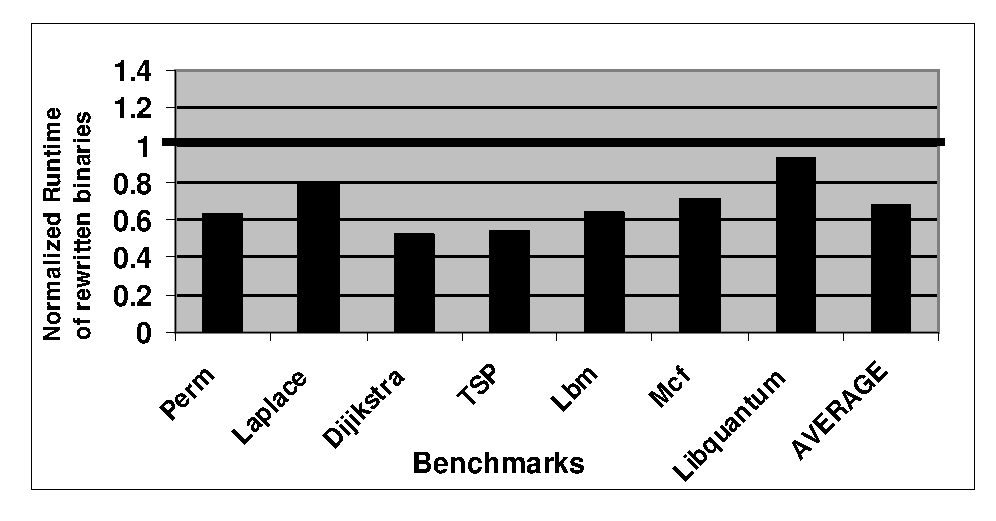
\includegraphics{perfunopt4}
\par\end{centering}
\renewcommand{\baselinestretch}{1}
\small\normalsize
\begin{quote}
\caption{Normalized runtime of rewritten binary as compared to input binary (runtime=1.0) that is
un-optimized}
\label{noopts}
\end{quote}
\end{figure}
\renewcommand{\baselinestretch}{2}
\small\normalsize

Figure \ref{noopts} shows the normalized run-time of each rewritten binary compared to an input
binary produced using GCC with no optimization (-O0 flag). We obtain an average improvement of 31\%
in execution time on our benchmarks with an improvement of over 40\% in some cases. This result
shows that our rewriter is useful for binaries that are not highly optimized, such as legacy
binaries from older compilers, or binaries from compilers that are inferior compared to the best
available compilers. In most cases, after rewriting we raised the performance close to that of an
optimized binary produced directly by GCC, showing the effectiveness of our approach.

Next, we study the performance of our rewriter on already optimized binaries. Figure \ref{withopts}
shows the normalized execution time of each rewritten binary compared to an input binary produced
using GCC with the highest available level of optimization (-O3 flag). In this case, the results are
mixed, with most benchmarks nearly breaking even or showing a small slowdown, one benchmark showing
a larger slowdown of 13\%, and one benchmark actually shows a speedup of 10\%. The average is 4\%
slowdown.

\begin{figure}
\begin{centering}
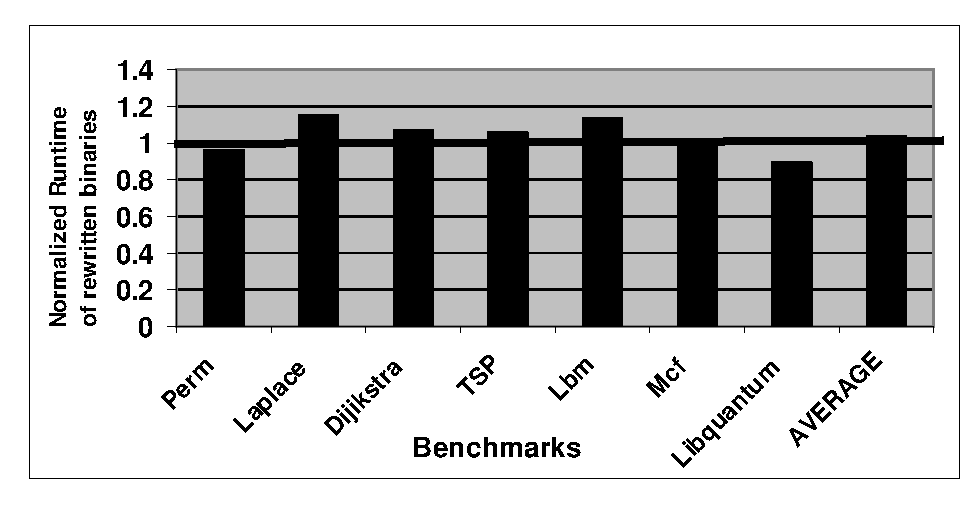
\includegraphics{perfopt4}
\par\end{centering}
\renewcommand{\baselinestretch}{1}
\small\normalsize
\begin{quote}
\caption{Normalized runtime of rewritten binary as compared to input binary (runtime=1.0) that is
optimized}
\label{withopts}
\end{quote}
\end{figure}
\renewcommand{\baselinestretch}{2}
\small\normalsize

We consider this near break-even performance on highly optimized binaries a good result for the
following three reasons: 

\begin{enumerate}

\item our initial goal was not necessarily to get a speedup, but to
generate correct IR without without introducing too much overhead. This would enable the IR to be a
starting point for various custom compiler transformations we wanted to perform thereafter, such as
automatic parallelization or security as covered in this thesis. Ultimately, these optimizations
determine the utility of the rewriter. 

\item these numbers represent our first cut implementation devoid of any attempt at producing a
better IR more geared towards optimization. We believe these numbers can be substantially improved
with more detailed IR and are exploring several related avenues. 

\item we have currently not implemented any custom serial optimizations that are likely to improve
performance further, such as the inter-procedural versions of common sub-expression elimination and
loop-invariant code motion, changing the compiler-enforced calling convention for registers for
better run-time, and more aggressive inlining. We believe these optimizations hold promise as the
inter-procedural optimization abilities of current compilers are very limited compared to their
intra-procedural performance.

\end{enumerate}

One additional advantage of the binary rewriter is that it accumlates optimizations accross two
compilers - rewritten binaries have an optimization if it is either present in the compiler that
produced the input binary, or in the rewriter. In our case, if either GCC or LLVM had an
optimization, the output binary should have it. This is why, for example, one of our rewritten
binaries (libquantum) had a 10\% speedup versus the input binary. Although GCC with the -O3
optimization flag is known to produce good code, in some cases it missed promoting structure fields
to registers whereas LLVM did, explaining the speedup in libquantum. With better IR and more
aggressive optimizations, we expect to see more consistent speedups in output binaries in the
future.

\subsection{Security Related Overheads}

We measured the overhead of the security schemes we implemented. These results are presented in
Figure \ref{secoverhead}. As seen the average overhead introduced is low at only 18\%. 

\begin{figure}
\begin{center}
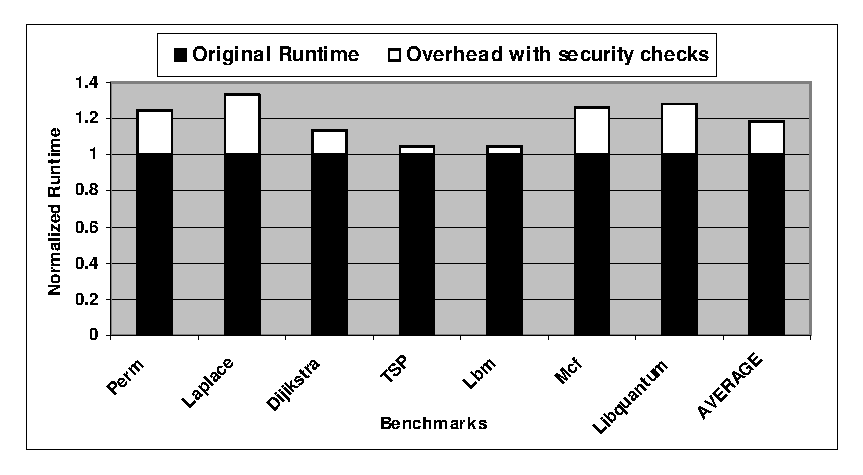
\includegraphics{security1.eps}
\end{center}
\renewcommand{\baselinestretch}{1}
\small\normalsize
\begin{quote}
\caption{Runtime overhead of rewritten binaries after inserting security checks.}
\label{secoverhead}
\end{quote}
\end{figure}
\renewcommand{\baselinestretch}{2}
\small\normalsize

\section{Real World Attacks}

Ultimately, the success of the scheme presented in this thesis is only valuable if it is applicable
to real-world attacks i.e. whether it can prevent attacks that have been observed in practice. In
this section, we reproduce a real-world attack and demonstrate that our rewriter halts this attack.

A HTTP server, GHTTPD, has a stack buffer overflow vulnerability in its logging function. We
produced an exploit for this server which overflows a stack-based buffer and corrupts the return
address.

Using the return address protection component of our scheme, we were able to rewrite the GHTTPD
server, add protection of the return address and prevent the attack which uses the buffer overflow
vulnerability to corrupt the return address. When our protection scheme is enabled, the return
address corruption is detected and the application is aborted.
